% This example is meant to be compiled with lualatex or xelatex
% The theme itself also supports pdflatex
\PassOptionsToPackage{unicode}{hyperref}
\documentclass[aspectratio=1610, 12pt, xcolor=dvipsnames]{beamer}

% Warning, if another latex run is needed
% \usepackage[aux]{rerunfilecheck}

% just list chapters and sections in the toc, not subsections or smaller
\setcounter{tocdepth}{1}

%------------------------------------------------------------------------------
%------------------------------ Fonts, Unicode, Language ----------------------
%------------------------------------------------------------------------------
\usepackage{fontspec}
\defaultfontfeatures{Ligatures=TeX}  % -- becomes en-dash etc.
\usepackage{multirow}
% german language
\usepackage{polyglossia}
\setdefaultlanguage{german}

% for english abstract and english titles in the toc
\setotherlanguages{english}

% intelligent quotation marks, language and nesting sensitive
\usepackage[autostyle]{csquotes}

% microtypographical features, makes the text look nicer on the small scale
\usepackage{microtype}

% colors and stuff
\usepackage{xcolor}
\usepackage[most]{tcolorbox}
\tcbset{on line, hbox,
        boxsep=4pt, left=0pt,right=0pt,top=0pt,bottom=0pt,
        colframe=white,colback=SpringGreen,
        highlight math style={enhanced}
        }
\newtcolorbox{mybox}[3][]
{
  colframe = #2!25,
  colback = #2!20,
  coltitle = #2!20!black,
  title = {#3},
  #1
}
%\colorlet{Green!40}
%------------------------------------------------------------------------------
%------------------------ Math Packages and settings --------------------------
%------------------------------------------------------------------------------

\usepackage{amsmath}
\usepackage{amssymb}
\usepackage{mathtools}
\usepackage{bbold}
\usepackage{hyperref}
\usepackage{url}

% Enable Unicode-Math and follow the ISO-Standards for typesetting math
\usepackage[
  math-style=ISO,
  bold-style=ISO,
  sans-style=italic,
  nabla=upright,
  partial=upright,
]{unicode-math}
\setmathfont{Latin Modern Math}

% nice, small fracs for the text with \sfrac{}{}
\usepackage{xfrac}


%------------------------------------------------------------------------------
%---------------------------- Numbers and Units -------------------------------
%------------------------------------------------------------------------------

\usepackage[
  locale=DE,
  separate-uncertainty=true,
  per-mode=symbol-or-fraction,
]{siunitx}
\sisetup{math-micro=\text{µ},text-micro=µ}
% \sisetup{tophrase={{ to }}}
%------------------------------------------------------------------------------
%-------------------------------- tables  -------------------------------------
%------------------------------------------------------------------------------

\usepackage{booktabs}       % \toprule, \midrule, \bottomrule, etc

%------------------------------------------------------------------------------
%-------------------------------- graphics -------------------------------------
%------------------------------------------------------------------------------

\usepackage{graphicx}
%\usepackage{rotating}
\usepackage{grffile}
\usepackage{tikz}
\usepackage{circuitikz}
\usepackage{tikz-feynman}
\usepackage{subcaption}

% allow figures to be placed in the running text by default:
\usepackage{scrhack}
\usepackage{float}
\floatplacement{figure}{htbp}
\floatplacement{table}{htbp}

% keep figures and tables in the section
\usepackage[section, below]{placeins}

% smileys
\usepackage{MnSymbol,wasysym}

%------------------------------------------------------------------------------
%---------------------- customize list environments ---------------------------
%------------------------------------------------------------------------------

\usepackage{enumitem}
\usepackage{listings}
\usepackage{hepunits}

\usepackage{pdfpages}
%------------------------------------------------------------------------------
%------------------------------ Bibliographie ---------------------------------
%------------------------------------------------------------------------------

\usepackage[
  backend=biber,   % use modern biber backend
  autolang=hyphen, % load hyphenation rules for if language of bibentry is not
                   % german, has to be loaded with \setotherlanguages
                   % in the references.bib use langid={en} for english sources
]{biblatex}
\addbibresource{references.bib}  % the bib file to use
\DefineBibliographyStrings{german}{andothers = {{et\,al\adddot}}}  % replace u.a. with et al.


% Load packages you need here
% \usepackage{polyglossia}
% \setmainlanguage{german}

\usepackage{csquotes}


% \usepackage{amsmath}
% \usepackage{amssymb}
% \usepackage{mathtools}

\usepackage{bookmark}

% load the theme after all packages

\usetheme[
  showtotalframes, % show total number of frames in the footline
]{tudo}

% Put settings here, like
\unimathsetup{
  math-style=ISO,
  bold-style=ISO,
  nabla=upright,
  partial=upright,
  mathrm=sym,
}

% \setbeamertemplate{itemize item}{\scriptsize$\blacktriangleright$}
% \setbeamertemplate{itemize subitem}{\scriptsize$\blacktriangleright$}

%Titel:
\title{Precision studies for 2024 SciFi Alignment}
%Autor
\author[N.Breer]{\textbf{Nils Breer} for the SciFi alignment team}
%Lehrstuhl/Fakultät
\institute{RTA: WP4/5 Alignment and Calibration}
%\titlegraphic{\includegraphics[width=0.3\textwidth]{content/Bilder/interferenz.jpg}}
\date{17.04.2025}

\begin{document}
\maketitle

\begin{frame}
  \begin{itemize}
    \item $\bullet$\, \textbf{Goal}: obtain precision of the SciFi alignment on 2024 data
  \end{itemize}
  Procedure:
  \begin{itemize}
    \item 1. Run alignment with a set configuration for several runs across multiple months
    \item 2. 200k events using the first run of each fill (if possible) on data starting at run 303874 (2024 alignment update in august)
    \item 3. Calculate the variation of each subsequent run w.r.t. the reference run
    \item 4. Histogrammed distributions per object, width as a metric for the precision
  \end{itemize}
  List of runs: 303963,304094,304191,304449,304528,304649,304802,304936,305071,305197,305291,305446,305498, \\
  305559,305641,305684,305850,306109,306356,306532,306608,306711,307071,30518,307587,307654,307758, \\
  307868,307897,307947,308073,308256
\end{frame}

\begin{frame}{Configurations}
  \begin{itemize}
    \item $\bullet$\, Config 1: CFrames Tx, Modules TxRz
    \item $\bullet$\, Config 2: CFrames Tx, Halfmodules Rx
    \item $\bullet$\, Config 3: CFrames Tx, Halfmodules TxRz
  \end{itemize}
  Constraints:
  \begin{itemize}
    \item $\bullet$\, Constraint to remove x-dependent translations and rotations (SxTx and SxRx) of modules in T3X2
    \item $\bullet$\, Halfmodule joint constraint
    \item $\bullet$\, z coordinate of module halves fixed to 0 on read-out edge
  \end{itemize}
\end{frame}

\begin{frame}\frametitle{Detectorposition in 2024, halfmodules TxRz alignment}
  \begin{itemize}
    \setlength\itemsep{0em}
    \item $\bullet$\, Halfmodules aligned in TxRz and CFrames in Tx
    \item $\bullet$\, Per layer, movement looks consistent over all runs \to expected
  \end{itemize}
  \begin{columns}
    \begin{column}[c]{0.5\textwidth}
      \begin{figure}
        \centering
        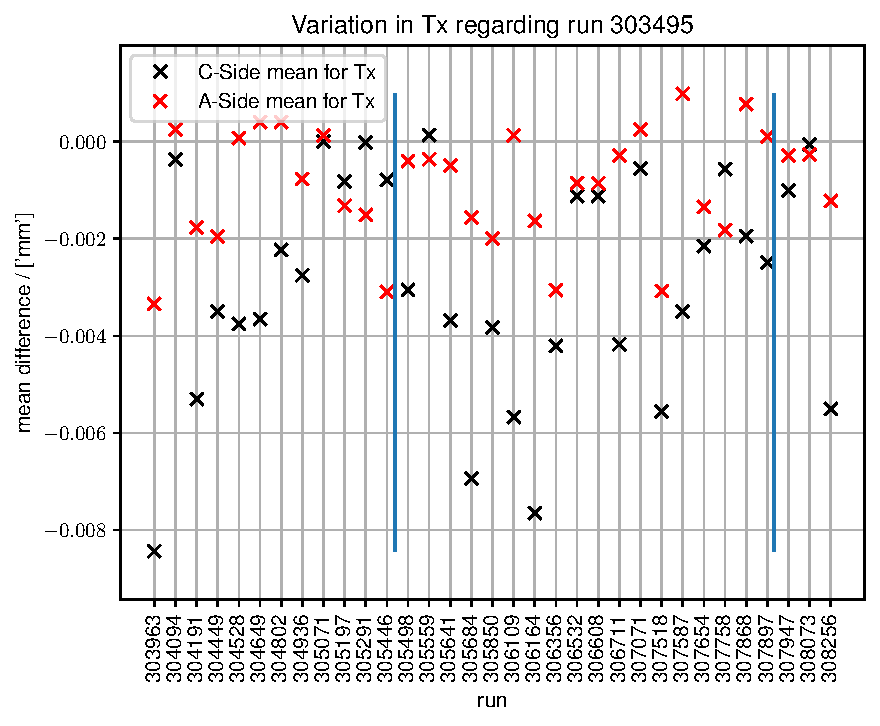
\includegraphics[width=0.8\textwidth]{plots/2025_plots_goettingen/scifi_stability_TxRz/half/stabi_test_Tx_half_correct.pdf}
      \end{figure}
    \end{column}
    \begin{column}[c]{0.5\textwidth}
      \begin{figure}
        \centering
        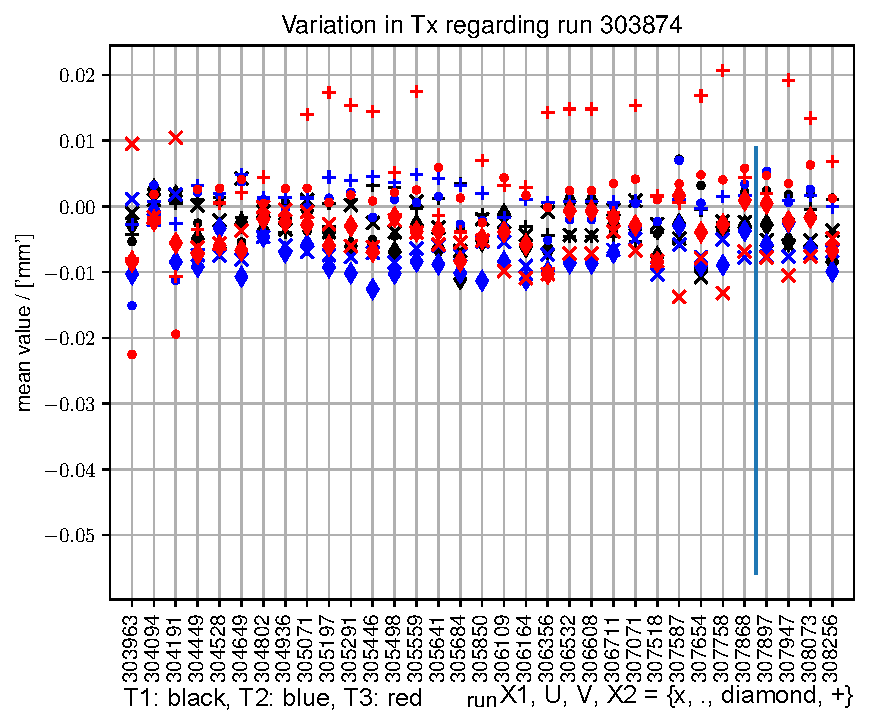
\includegraphics[width=0.8\textwidth]{plots/2025_plots_goettingen/scifi_stability_TxRz/per_layer/stabi_test_Tx_per_layer.pdf}
      \end{figure}
    \end{column}
  \end{columns}
\end{frame}

\begin{frame}\frametitle{Config 3: CFrames Tx}
  \begin{columns}
    \begin{column}[c]{0.33\textwidth}
      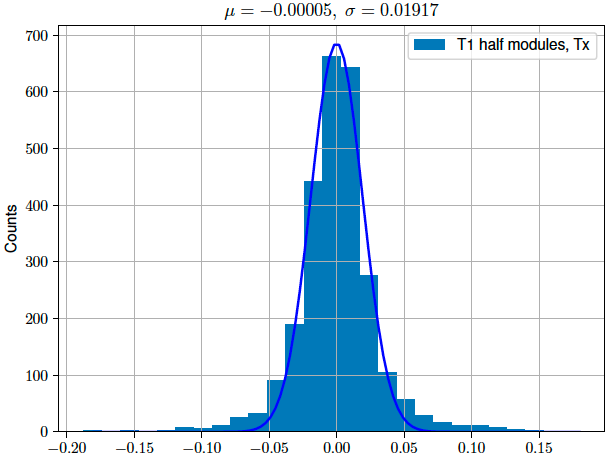
\includegraphics[width=\textwidth]{plots/2025_plots_precision/T1.png}
      Station 1
    \end{column}
    \begin{column}[c]{0.33\textwidth}
      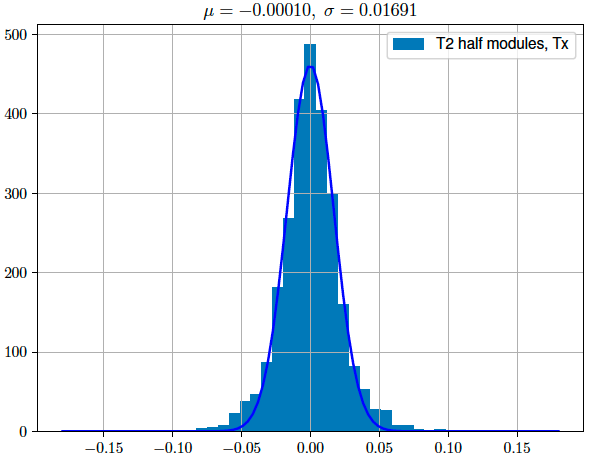
\includegraphics[width=\textwidth]{plots/2025_plots_precision/T2.png}
      Station 2
    \end{column}
    \begin{column}[c]{0.33\textwidth}
      WIth M5 modules included
      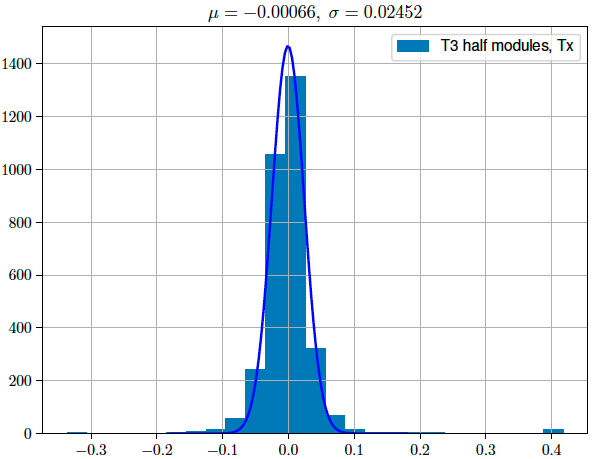
\includegraphics[width=\textwidth]{plots/2025_plots_precision/T3.png}
      Station 3
    \end{column}
  \end{columns}
\end{frame}

\begin{frame}\frametitle{Config 3: CFrames Rz}
  \begin{table}
    \begin{tabular}{c | c}
      \toprule
        Station & Rz width [$\mu$rad] \\
      \midrule
        T1 & 13.5 ± 0.2 \\
        T2 & 12.4 ± 0.2 \\
        T3 & 18.4 ± 0.3 \\
      \bottomrule
    \end{tabular}
  \end{table}
  \begin{columns}
    \begin{column}[c]{0.33\textwidth}
      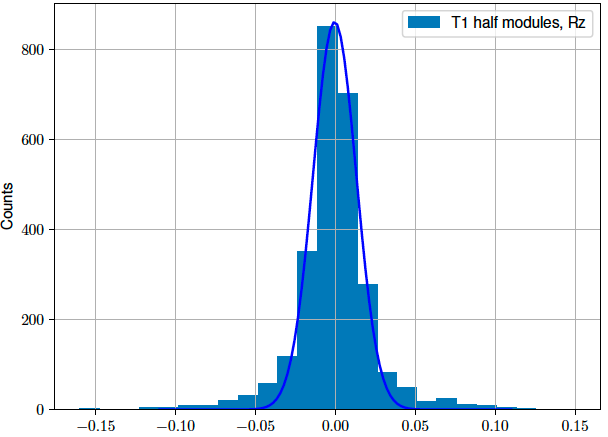
\includegraphics[width=\textwidth]{plots/2025_plots_precision/T1_Rz.png}
      Station 1
    \end{column}
    \begin{column}[c]{0.33\textwidth}
      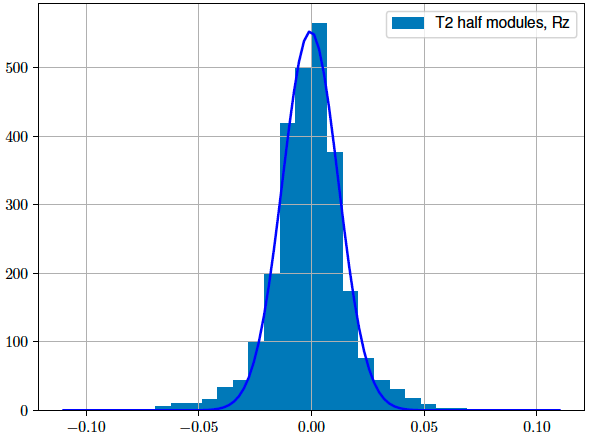
\includegraphics[width=\textwidth]{plots/2025_plots_precision/T2_Rz.png}
      Station 2
    \end{column}
    \begin{column}[c]{0.33\textwidth}
      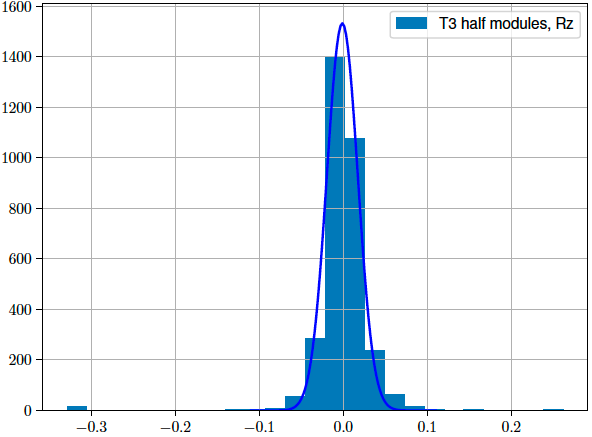
\includegraphics[width=\textwidth]{plots/2025_plots_precision/T3_Rz.png}
      Station 3
    \end{column}
  \end{columns}
\end{frame}

\begin{frame}
  CFrames Tx (values in $\mu$m)
  \begin{table}
    \begin{tabular}{c | c c c}
      \toprule
         & T1 & T2 & T3 \\
      \midrule
        2024 data & 19.2 ± 0.3 & 16.9 ± 0.3 & 24.5 ± 0.4 \\
        MC        & 16.5 ± 0.1 & 19.8 ± 0.2 & 37.0 ± 0.5 \\
      \bottomrule
    \end{tabular}
  \end{table}
  Values grouped by Modules
  \begin{table}
    \begin{tabular}{c | c | c c c c c c}
      \toprule
        & & M0 & M1 & M2 & M3 & M4 & M5 \\
      \midrule
      \multirow{2}{3em}{Tx [$\mu$m]} & 2024 data & 17.8 ± 0.4 & 15.3 ± 0.4 & 14.2 ± 0.3 & 21.1 ± 0.5 & 32 ± 0.8 & 39.9 ± 1.7 \\
                            & MC & 22.0 ± 0.4 & 22.4 ± 0.4 & 21.2 ± 0.4 & 17.4 ± 0.1 & 27.2 ± 0.3 & 135 ± 3 \\
      \hline
      \multirow{2}{3em}{Rz [$\mu$rad]} & 2024 data & 9.8 ± 0.2 & 10.8 ± 0.2 & 12.8 ± 0.3 & 15.1 ± 0.4 & 27.1 ± 0.7 & 39.1 ± 1.7 \\
                            & MC & 15.3 ± 0.5 & 16.6 ± 0.3 & 16.0 ± 0.2 & 12.8 ± 0.2 & 8.5 ± 0.3 & 44 ± 1 \\
      \bottomrule
    \end{tabular}
  \end{table}
\end{frame}

\begin{frame}\frametitle{Conclusion}
  \begin{itemize}
    \item $\bullet$\, Good sensitivity to align modules and CFrames and we are below the single hit resolution \approx 100 $\mu$m
    \item $\bullet$\, Results are comparable with MC-simulated data
    \item $\bullet$\, CFrame precision is station dependent \to set a high enough threshold for all stations or set separate thresholds per station
    \item $\bullet$\, For values on MC-simulated data see Miguel's slides \href{https://indico.cern.ch/event/1475162/contributions/6240307/attachments/2976257/5239245/Alignment_precision_WP4.pdf}{here}
    \item $\bullet$\, the full documentation of the SciFi alignment in run 3 including these stability studies will be in the internal note
    \item $\bullet$\, stability study plots: /Documents/promotion/scifi-stability-...
  \end{itemize}
\end{frame}

\begin{frame}\frametitle{Followup work}
  \begin{itemize}
    \item $\bullet$\, do more runs with TxTzRz for CFrames (also add VELO global constants in the Alignment)
    \begin{itemize}
      \item $\bullet$\, Will need to check the constants. 
      \item $\bullet$\, LBRunDB check runs i can use
      \item $\bullet$\, Also aligning Halflayers in Tz is satisfying the "most important degrees of freedom" -> no Rz in the modules
      \item $\bullet$\, Have to do at least 50 more runs -> when doing fit per station do 1 combining this config with what i already have and 1 fit with only the new constants
    \end{itemize}
  \end{itemize}
\end{frame}

\begin{frame}\frametitle{Followup work}
  \begin{itemize}
    \item $\bullet$\, /Users/nibreer/Documents/promotion/Alignment/Alignment/AlignmentMonitoring/rootmacros
    \item $\bullet$\, Here ic can use 
    \item forge
    \item root
    \item root> .L drawutils.cxx
    \item root> .L drawalignment.cxx
    \item root> drawall( "before alignment:Iter0/GoodLongTracks_histo.root","after alignment:Iter5/GoodLongTracks_histo.root")
    \item put the correct path to the files instead of Iter0 ...
  \end{itemize}
\end{frame}

\begin{frame}\frametitle{Followup work}
  adding more plots to wouter's plotting script
  \begin{itemize}
    \item $\bullet$\, path from above in drawalignmon
    \item $\bullet$\, add an additional monitor at the top if needed
    \item $\bullet$\, add new page like this: monapp->addPage( new MonitoringPage('example page', monitor + plot_from_root_file, ...))
    \item $\bullet$\, outputfile: all_maps2.pdf
    \item $\bullet$\, fix stack -> use_iosvc is not in it -> /LHCb/.../application.py
    \item $\bullet$\, /calib/align/LHCb/Muon -> Jpsi data, /calib/align/LHCb/Tracker -> D0 data
  \end{itemize}
\end{frame}

\begin{frame}\frametitle{may 2025 work}
  \begin{itemize}
    \item $\bullet$\, used first 2025 data on Jpsi (Muon path) to get this results: /swdev/nibreer/align_output/2025/first_2025_test/conf1_tracker_0510_released_Tx_constr
    \item $\bullet$\, conf2 looks better than conf1 see my plots in alignment mattermost from 10th may
    \item $\bullet$\, residuals and matching plots are improved
    \item $\bullet$\, for tomorrow, sunday 11th may 2025 we plan to update the constants to the config 2 ones
    \item $\bullet$\, VELO: it is actually the modules that move (stand: 13th may 2025)
    \item $\bullet$\, For me: run config 2 from the fill from last night (without the first run since it still has VELO drift)
    \item $\bullet$\, i was using swdev31: check this maschine if i need the commands for the tmux sessions
  \end{itemize}
\end{frame}

\end{document}
